%--------------------
% Packages
% -------------------
\documentclass[11pt,a4paper]{article}
\usepackage[utf8]{inputenc}
\usepackage[T1]{fontenc}
\usepackage{mathptmx} % Use Times Font


\usepackage[pdftex]{graphicx} % Required for including pictures
\usepackage[english]{babel}
\usepackage[pdftex,linkcolor=black,pdfborder={0 0 0}]{hyperref} % Format links for pdf
\usepackage{calc} % To reset the counter in the document after title page
\usepackage{enumitem} % Includes lists
\usepackage{booktabs}
\usepackage{longtable}
\usepackage{chngpage}

\usepackage{csquotes}
\usepackage[
backend=biber,
style=apa,
sorting=ynt
]{biblatex}
\addbibresource{bibliography.bib}

\frenchspacing % No double spacing between sentences
\linespread{1.2} % Set linespace
\usepackage[a4paper, lmargin=0.1666\paperwidth, rmargin=0.1666\paperwidth, tmargin=0.1111\paperheight, bmargin=0.1111\paperheight]{geometry} %margins
%\usepackage{parskip}

\usepackage[all]{nowidow} % Tries to remove widows
\usepackage[protrusion=true,expansion=true]{microtype} % Improves typography, load after fontpackage is selected

%-----------------------
% Set pdf information and add title, fill in the fields
%-----------------------
\hypersetup{
pdfsubject = {},
pdftitle = {},
pdfauthor = {}
}

%-----------------------
% Begin document
%-----------------------
\begin{document}

\section{Acknowledgements}

The author acknowledges the IT University of Copenhagen HPC resources made available for conducting the research reported in this paper.

\section{Introduction}

\section{Related Work}

Traditionally readability in texts is usually measured using a formula that
considers certain features of the text. This is commonly features such as
average sentence length and average number of syllables per word in the text.
One of the most commonly used measure of readability of English texts is the
Flesch Reading Ease (FRE), which is based on those two features. It was developed by
Rudolf Flesch in the 1940s and is still widely used today and is used as the US
government standard. Another widely used metric of readability is the Flesch-Kincaid reading grade level. This was
developed by J. Peter Kincaid in 1975 and is a development on the Flesch
reading ease intended to make it easier to use. The Flesch reading ease
produces a number from 0-100. Various ranges of the score can be interpreted as
corresponding to certain US grade levels. While the Flesch-Kincaid reading
grade level formula produces a score that directly corresponds to a US grade
level.

About 20 years ago research into automatic classification of readability levels
started to be done. One of the big downsides to the classical readability
formulas is that they require certain assumptions for the text in order to work
well. One of these is that the text must contain at least 100 words or 10
sentences, and that it uses well defined sentences such that sentence length
can be properly measured. Particularly the limitation on sentence length led to
two of the first studies into automatic classification of readability.
\parencite{collins-thompson-callan-2004-language}
use a multinomial naïve Bayes model that combines multiple language models to
estimate the most likely grade level for any given passage.
\parencite{10.1145/1008992.1009114} use support vector machine learning algorithms
based on both syntactic and semantic features and treat the readability
estimation as a text classification problem.

Automatic classification of readability has some benefits over the traditional
formulas typically used for readability estimation. The main one that was the
drive behind the studies mentioned is accuracy on shorter texts. But
additionally the use of trained classifiers means that it is possible to train
or re-train models for specific purposes.
\parencite{collins-thompson-callan-2004-language} show that they obtain good
performance for both English and French, only requiring a change in morphology
handling during feature processing. A recent study has also looked at using
automatic classification of readability, specifically on the CEFR scale.
\parencite{kerz-etal-2021-automated} use RNNs combined with a sliding window
technique to predict CEFR levels.

\section{Data}

\subsection{Training Dataset}

The training data come from the Education First Cambridge Open Language
Database (EFCAMDAT) \parencite{inbook}. The database
contains user submitted texts from EF Education First, an international English school teaching English as a second language. The database is compiled
in collaboration with Cambridge University \parencite{hgbka17}. The database
contains student assignment submission to Englishtown, which is the online
school of EF Education First. Students submit assignments that are graded and
error corrected by a teacher. The grade is included in the data, as is the
error corrections for a portion of the assignments. The curriculum of
Englishtown is split into 16 levels, which cover all six CEFR levels from A1
to C2. The relation between the Englishtown levels and CEFR levels is shown in
\autoref{tab:englishtown-cefr}. The database release contains a subcorpus which contains the texts that
have error corrections supplied (Öksüz et al., paper unavailable as it is under
review). The error corrections have been applied to the texts to produce
corrected texts. The full database contains 1,180,309 submissions and the
subcorpus contains 620,207 of these with automatically corrected texts. There
is a rather uneven distribution of CEFR labels in the subcorpus as can be seen
in \autoref{fig:efcamdat-distribution}. Additionally, no texts from the C2 level
are included in the subcorpus used for training the model. Some examples of
sentences from assignment texts can be seen in \autoref{tab:efcamdat-examples}.

\begin{table}
  \centering
  \begin{tabular}{l|cccccc}
    \toprule
    Englishtown & 1-3 & 4-6 & 7-9 & 10-12 & 13-15 & 16 \\
    \midrule
    CEFR & A1 & A2 & B1 & B2 & C1 & C2 \\
    \bottomrule
  \end{tabular}
  \caption{Englishtown levels in relation to CEFR levels}
  \label{tab:englishtown-cefr}
\end{table}

\begin{table}
  \centering
  \begin{tabular}{l|p{0.85\linewidth}}
    \toprule
    Level & Text  \\
    \midrule
    1 & Hi, everyone. This is the menu: Starter: Vegetables and cheese. Main
    course: Chicken and rice. Dessert: Ice cream. See you soon.\\
    \midrule
    8 & Hi Mr. Smith, I'd like to inform you that I have recently had a meeting
    with our business partner, Sally Cassidy. She was very friendly and
    optimistic. We discussed our cooperative project for the next year. It
    seems like a very lucrative and meaningful one. It's imperative to wrap up
    our current manufacturing process, so that we will be able to start the new
    one. (...)\\
    % Sally Cassidy invited me to visit their office and speak about the
    % schedule tomorrow morning. However, I will keep you informed. Best regards,
    % Tatiana\\
    \midrule
    15 & Last year I was on a vacation in California. It was wonderful but
    one thing stays in my mind. People in America tend to communicate more
    indirectly compared with people in Germany, where I'm living. If you talk
    with someone you don't know you don't know if he says the truth or just
    wants to be nice to you. Sometimes this is really strange. (...)\\
    % But this is a
    % foreign country with a different culture than what we have in Germany.
    % Nevertheless I prefer direct communication although it's vulnerable. The
    % kind of body language is similar to the one in Germany. There are no big
    % differences.\\
    \bottomrule
  \end{tabular}
  \caption{Example of texts from EFCAMDAT subcorpus at certain Englishtown levels}
  \label{tab:efcamdat-examples}
\end{table}

\begin{figure}
  \centering
  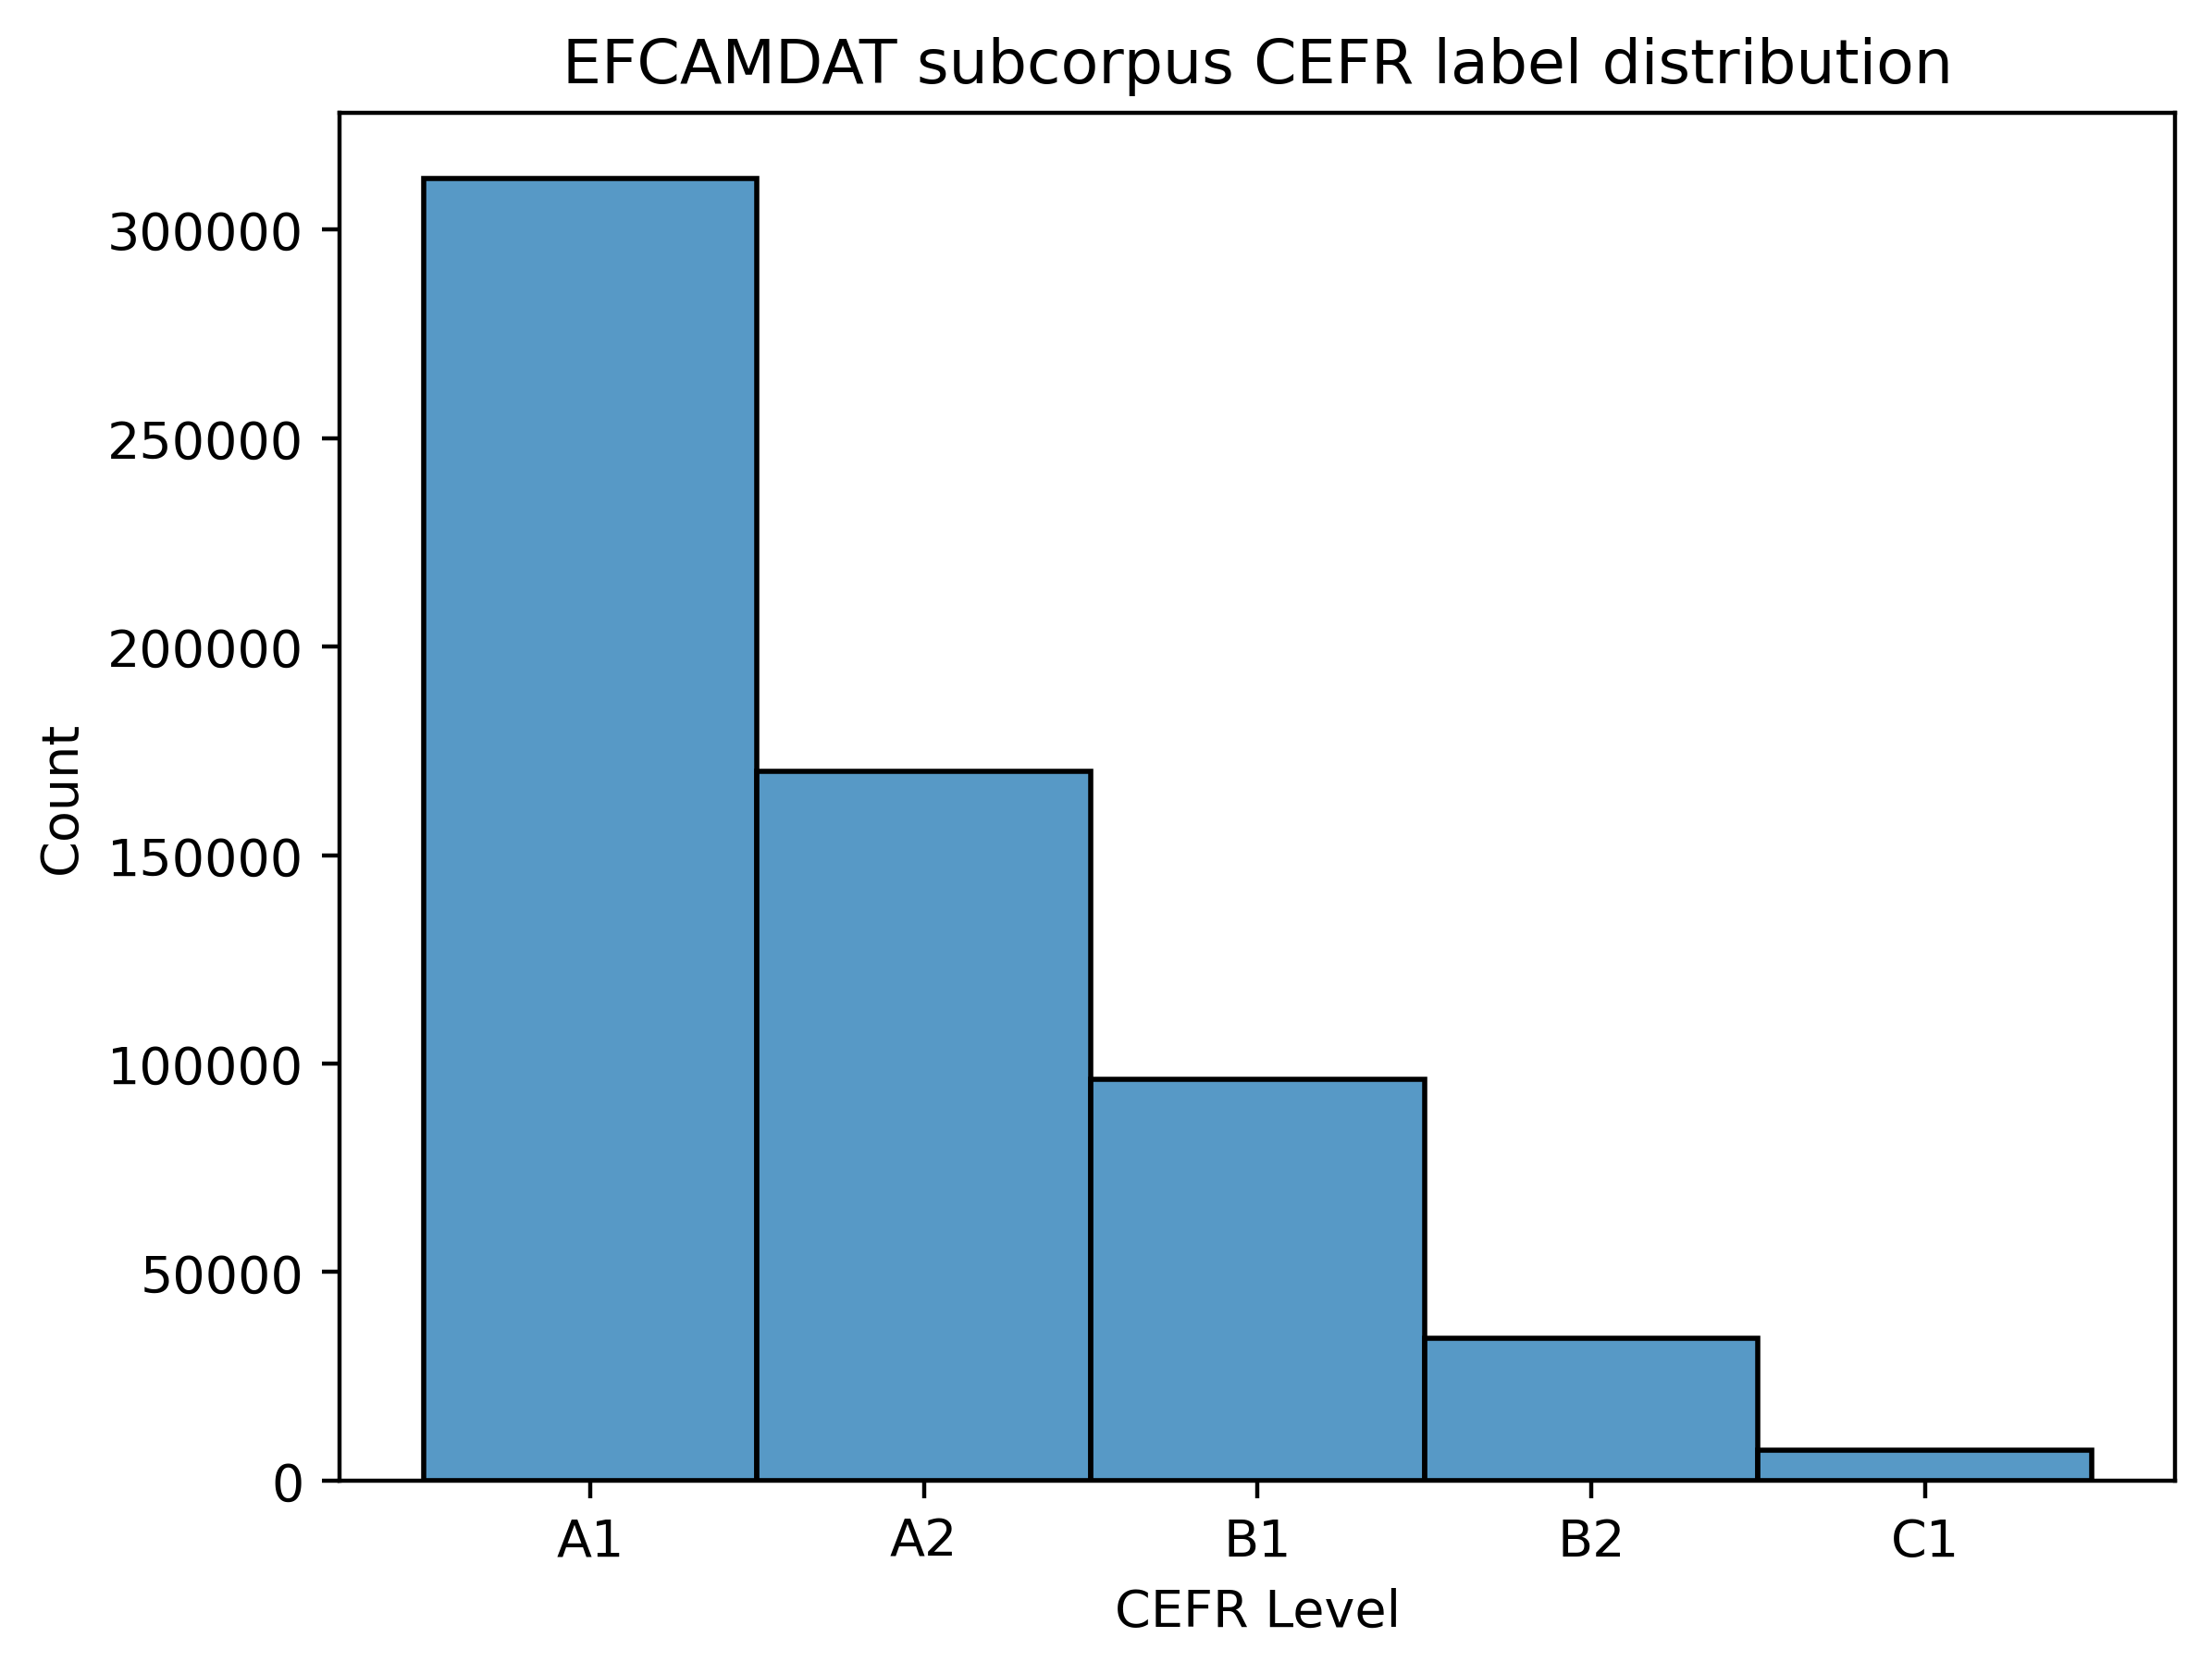
\includegraphics[width=0.8\textwidth]{figures/cefr-distribution-efcamdat.png}
  \caption{Distribution of CEFR levels for EFCAMDAT subcorpus}
  \label{fig:efcamdat-distribution}
\end{figure}

\subsection{Validation Dataset}

For use in validating the performance of the trained model, I compiled a
validation corpus of texts from English teaching books at each CEFR level.
All books are from different book series all from National Geographic Learning.
For an overview of the specific book title used for each CEFR level see
\autoref{tab:validation-books}. All the books have a pretty similar structure
consisting of exercises where the reader must fill in or pick the right
word(s), multiple choice questions, and reading comprehension questions. The
reading comprehension questions are all accompanied by a text of varying
length. Some are a couple sentences long, while others span multiple
paragraphs. Some examples of texts at different CEFR levels can be seen in
\autoref{tab:validation-examples}. I collected all of these texts from each book to use for the
validation corpus. To extract the texts from the books, I scanned the books and
did OCR using \verb!pytesseract! to
extract the text. I then manually went through and corrected each scanned text,
as the text was not always extracted correctly.

The assumption is that since each book is stated to be
intended for at a specific CEFR level of proficiency, the texts from the
reading comprehension exercises should be at that level of readability. The
result is a corpus with CEFR labeled texts that can be used to validate the
model. The distribution of labels in the resulting corpus is more even than in
the training data, with many more difficult texts, as can be seen in
\autoref{fig:validation-distribution}.

\begin{table}
  \centering
  \begin{tabular}{r|l}
    \toprule
    CEFR Level & Book Title\\
    \midrule
    A1 & English Explorer 1\\
    A2 & Close Up A2\\
    B1 & World English 3\\
    B2 & Perspectives Upper Intermediate\\
    C1 & Perspectives Advanced\\
    C2 & Close Up C2\\
    \bottomrule
  \end{tabular}
  \caption{Books used for validation corpus}
  \label{tab:validation-books}
\end{table}

\begin{table}
  \centering
  \begin{tabular}{l|p{0.85\textwidth}}
    \toprule
    CEFR & Text\\
    \midrule
    A1 & My name's Annie Twigg and I'm a scientist. The chimpanzees in the photo are
    from Africa. They're a family. They're brothers and sisters. Their names
    are Tom, Brad, Keira and Angelina. They're happy. Their mother is in the
    photo too. Her name’s Meryl.\\
    \midrule
    B1 & My name is Richard. All my life, I lived in New York City, but when I
    retired five years ago, I moved to Florida. I love it here! It’s sunny and
    beautiful every day of the year—and that means I can play golf every day.
    Golf is my favorite thing in life. I'm not far from the ocean, and I can go
    to the beach any time I want. It’s too bad that my children are all so far
    away, but they can visit me any time they want to. This is the perfect life
    for me!\\
    \midrule
    C2 & Peer pressure exists across society, affecting people beneficially and adversely.
    In the case of the latter, certain risk factors have been identified that can make
    young people prone to undue, and often unwelcome, influence. When this occurs,
    there are strategies that can be used to handle the problem.
    Peers play an important role in a teenager's life as adolescence is the time
    when the desire to fit in and find acceptance and approval from the group is
    strongest. (...)\\
    % The need for approval is not bad in itself. It is part of what
    % motivates adolescents to take extra care with their appearance, for instance.
    % At times however, the desire to either impress or gain acceptance by the group
    % becomes excessive, and can result in people choosing to take risks, with
    % potentially serious consequences. Similarly, they might engage in behaviour
    % that is extremely hurtful, like ridiculing someone with a physical or mental
    % disability\\
    \bottomrule
  \end{tabular}
  \caption{Example of texts from validation corpus}
  \label{tab:validation-examples}
\end{table}

\begin{figure}
  \centering
  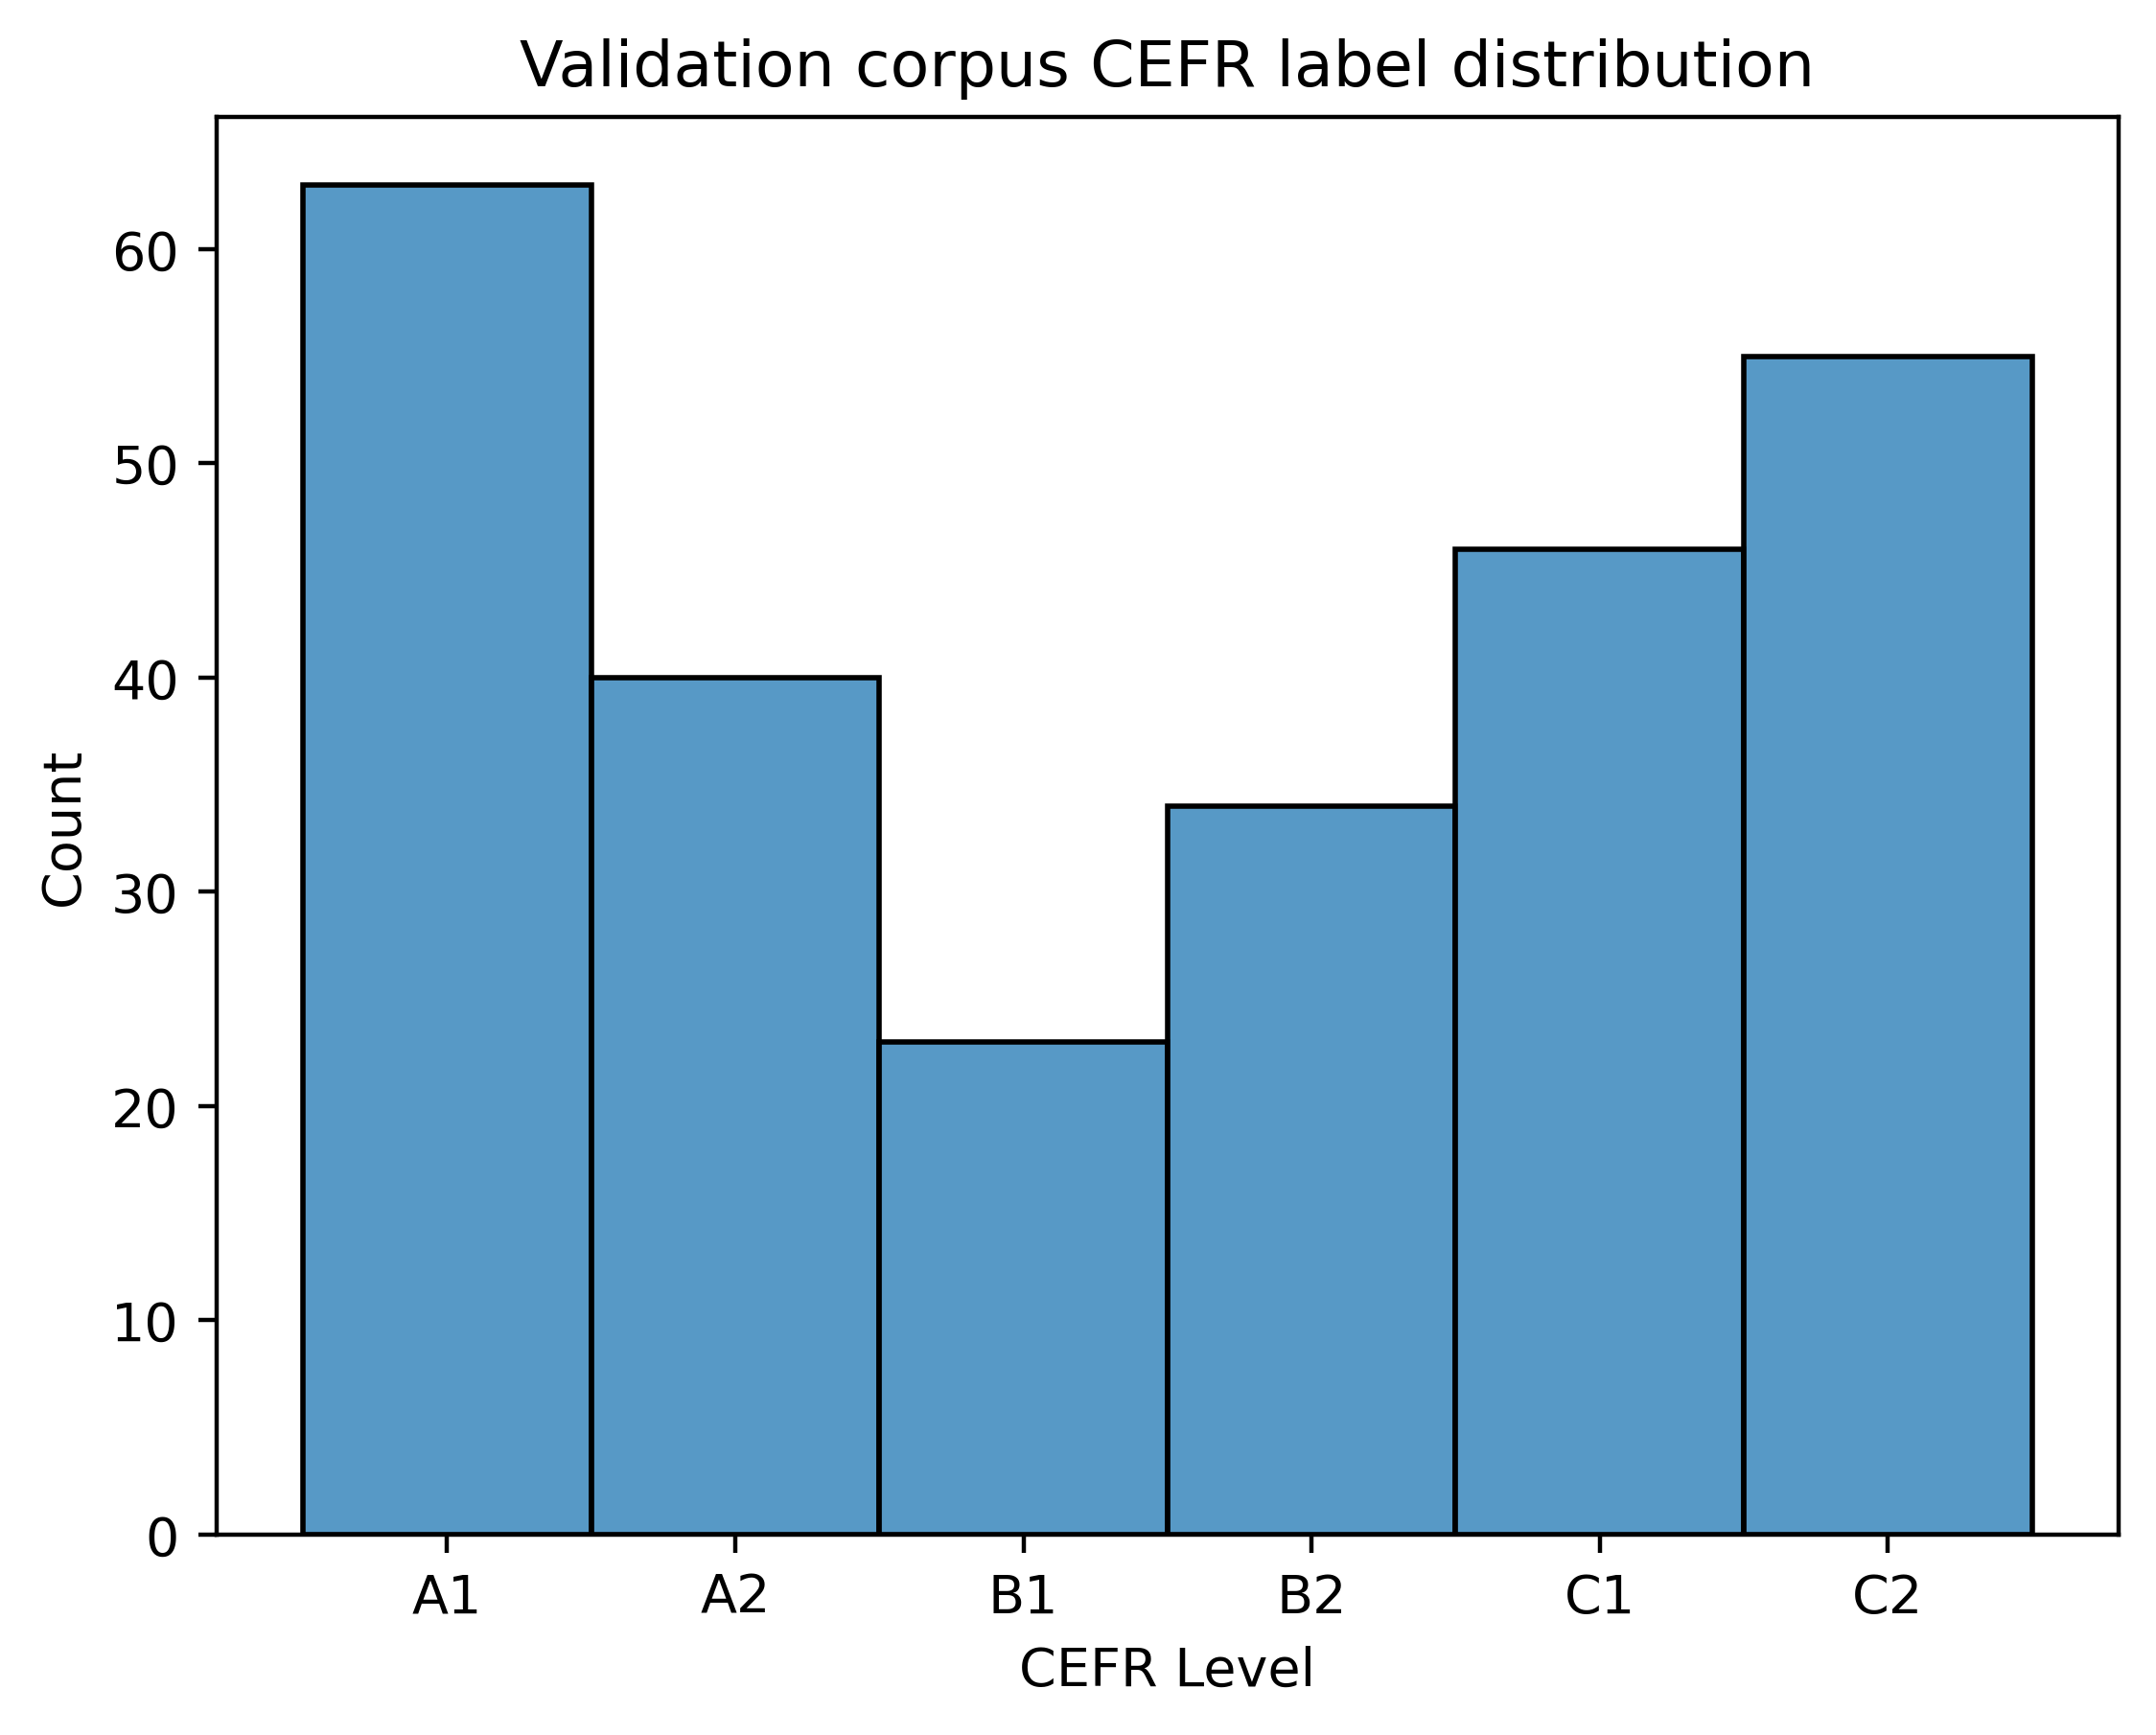
\includegraphics[width=0.8\textwidth]{figures/cefr-distribution-validation.png}
  \caption{Distribution of CEFR levels for validation corpus}
  \label{fig:validation-distribution}
\end{figure}

\section{Methodology}

I trained multiple models on the EFCAMDAT subcorpus. Some were trained using the
texts as they are, but I also trained a model using a windowing technique
similar to \parencite{kerz-etal-2021-automated}. In the following sections I
will describe the setup and methodology used in training and evaluating each
set of models.

\subsection{Dataset splitting}

For training the models without the windowing technique, the whole EFCAMDAT subcorpus was split
into train, evaluation, and test splits. This was done using random sampling.
The training set was given 80\% of the data, with the evaluation and training
sets each containing 10\% of the data. As illustrated in
\autoref{fig:dataset-splits-labels}, the result is that each split of data has
a nearly identical distribution of labels. I did not convert the Englishtown
levels into CEFR before training the models, so all models output the 1-16
Englishtown levels which can then be converted into CEFR.

\begin{figure}
  \centering
  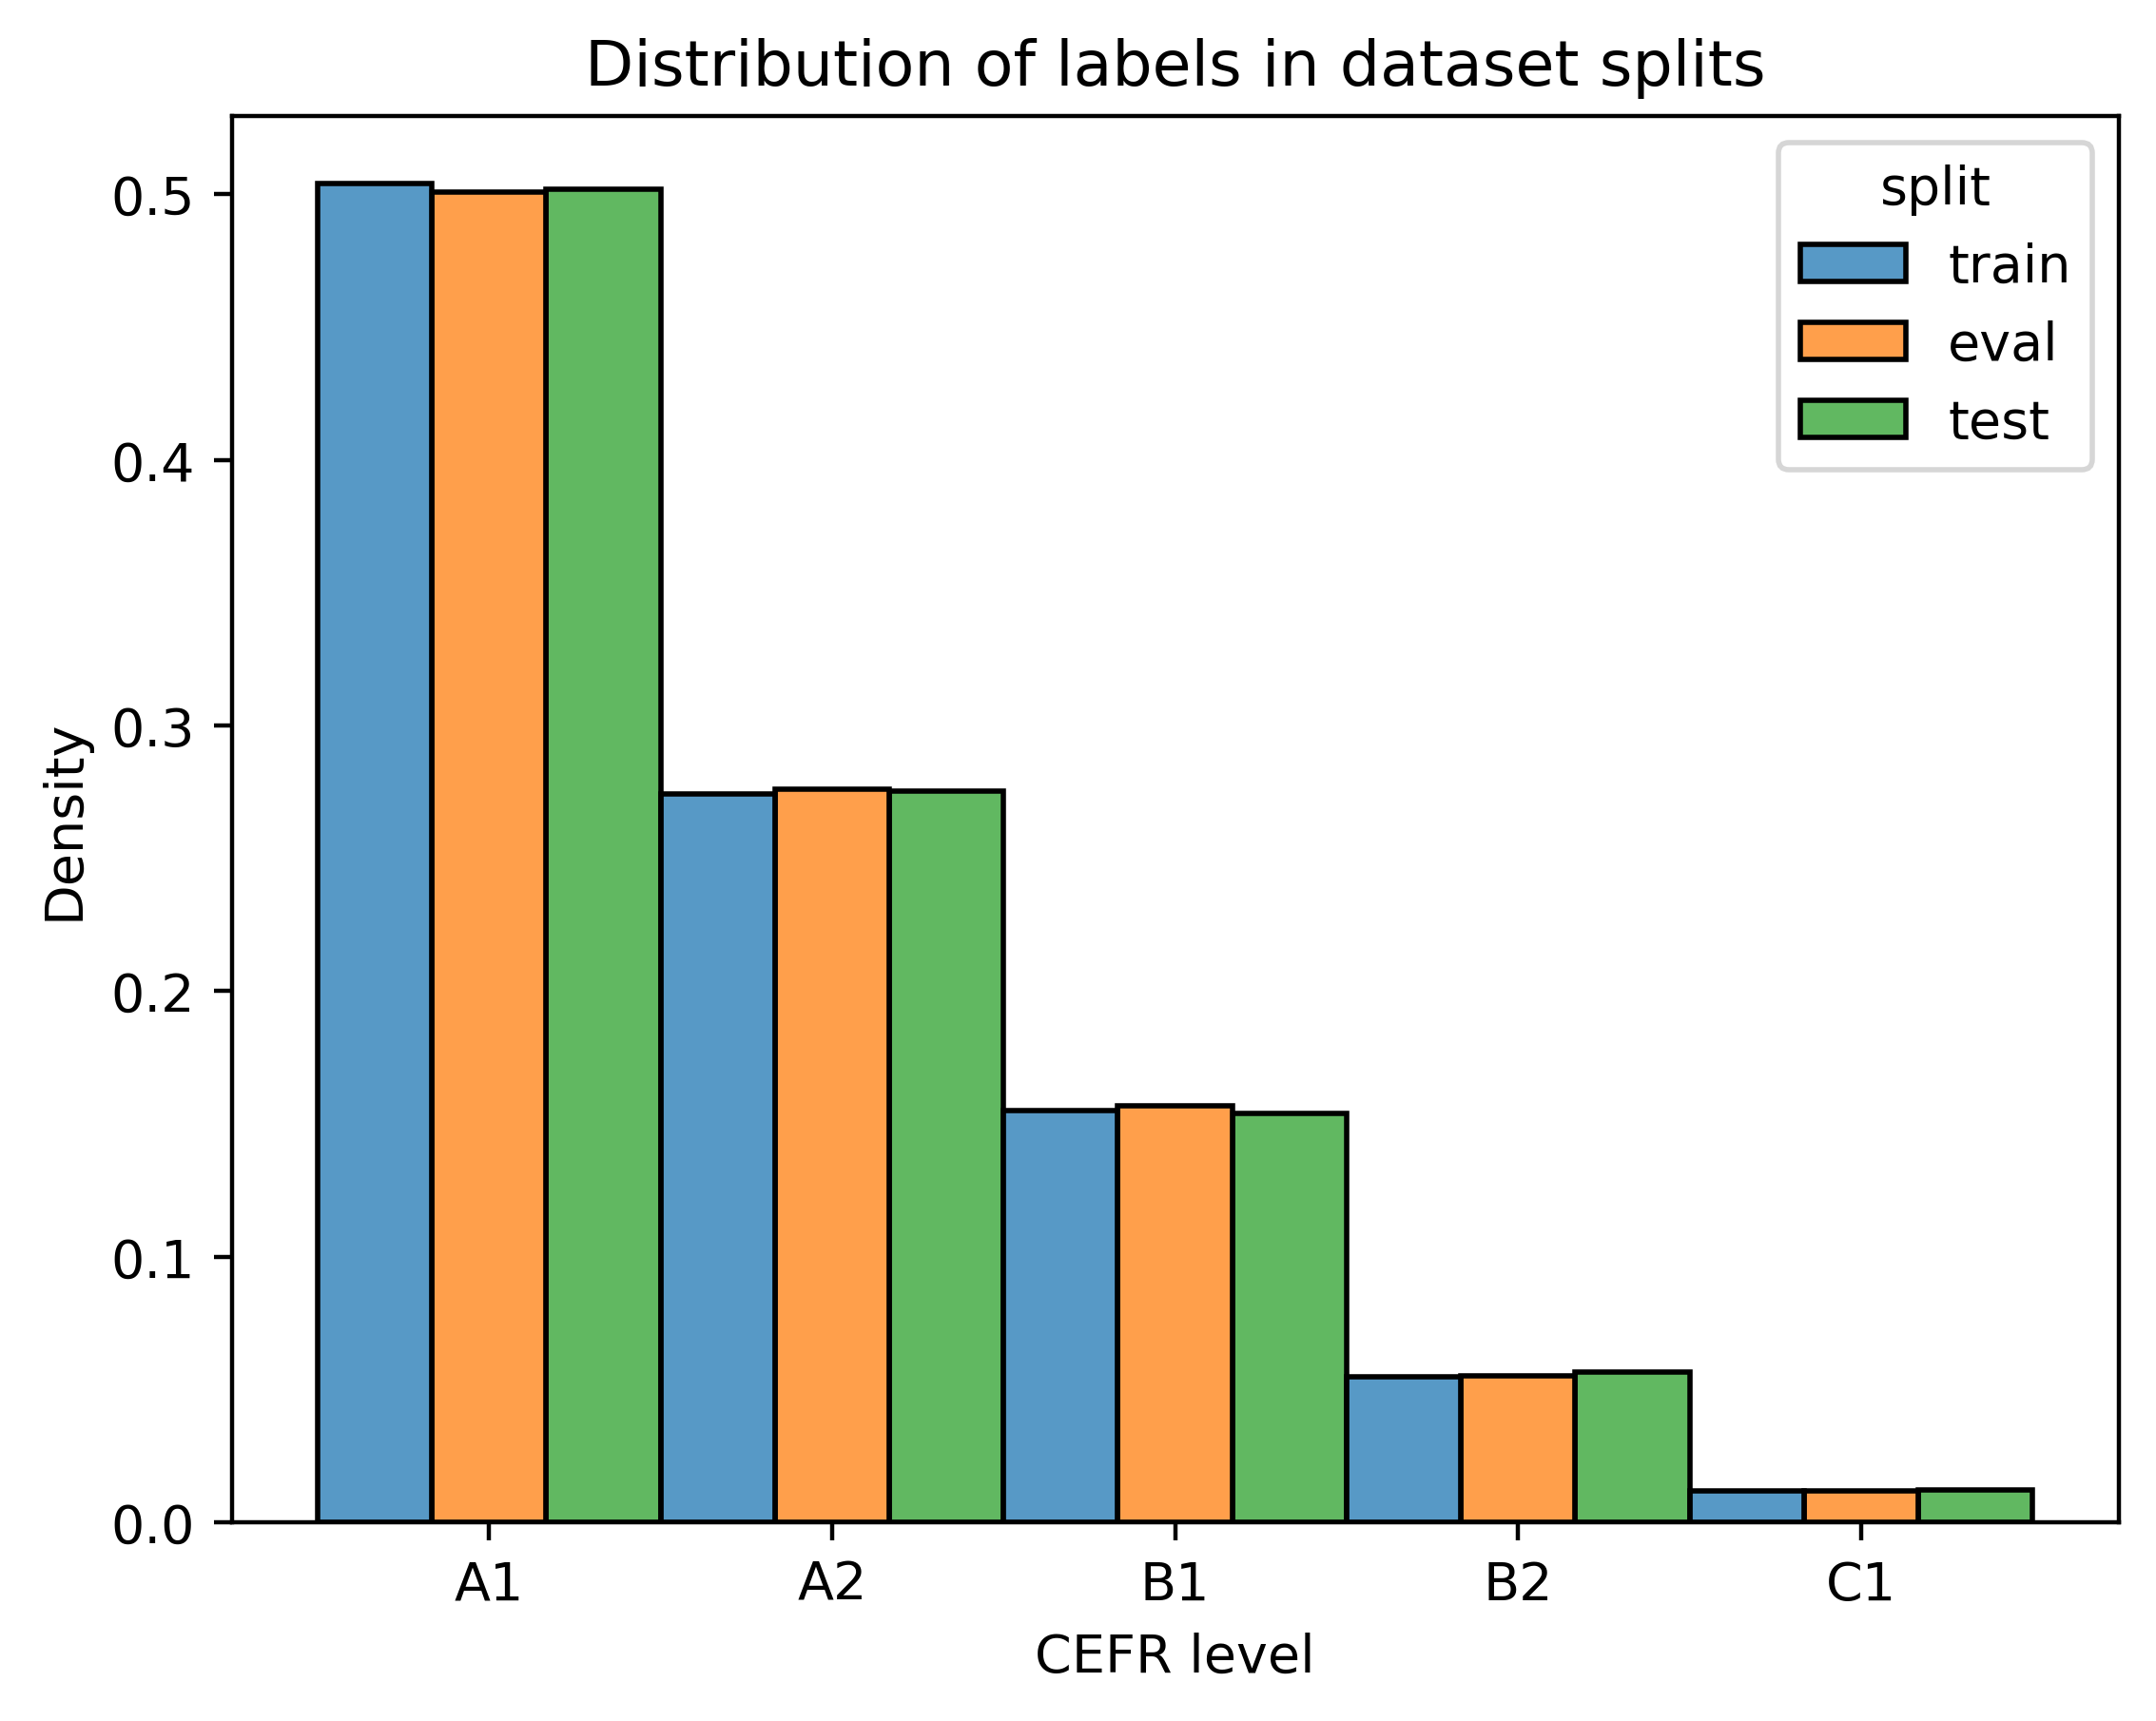
\includegraphics[width=0.7\textwidth]{figures/split-distributions-full-texts.png}
  \caption{CEFR label distribution in dataset splits}
  \label{fig:dataset-splits-labels}
\end{figure}

\subsection{Simple SVM models}

I trained a some simple support vector machine (SVM) models on surface level features in the
train split of the dataset. The features used were average sentence length and
term frequency-inverse document frequency (TF-IDF). I trained three models, two
using each feature separately and one using both in combination. The models
were trained using \verb!sklearn!'s \verb!SGDClassifier! which trains an SVM
model using stochastic gradient descent (SGD) learning and default parameters. As part of
preprocessing the features were standardized. In the model using only sentence
length the data was standardized to unit mean and variance. In the two models
using TF-IDF the data was only standardized to unit variance, as the very
sparse nature of the TF-IDF feature matrix made it impossible to standardize
the mean.

\subsection{BERT model without windowing}

I also trained a BERT model on the train split of the dataset. The model was trained
using the \verb!Trainer! class from the \verb!transformers! package, and the
model used was the \verb!google-bert/bert-base-cased! model. The model was
trained using default parameters and with accuracy used for early stopping.
The evaluation split was used to compute the accuracy for early stopping.

\subsection{BERT model using windowing technique}

I additionally trained a BERT model using a windowing technique on the training
split. Instead of each piece of training data being a full text and the
corresponding label, the text is split into multiple data points by using a
sliding window. The window used corresponds to about 3 sentences. I computed
the median sentence length in the dataset to be approximately 12.5 words and
the average word length to be approximately 4 characters. By using a window
size of 150 characters, that is equivalent to 3 sentences based on those median
measurements. The sliding window starts at the beginning of the text and
captures the next 150 characters. Then it moves to the beginning of the second
sentence, takes the next 150 characters. Then it moves to the beginning of the
third sentence, and so on until there are no more sentences in the text. An
example of how this looks for a sample text is shown in
\autoref{tab:windowing-example}. The idea behind using the windowing technique
is to prevent the model from fitting to closely on just the length of the whole texts
as well as the sentence lengths.

The result is that there are was a lot more training data after applying the
windowing to the dataset. To keep the training time within a realistic time frame, is was
necessary to thin out the dataset by sampling some of it. I aimed to even out
the distribution of labels in the dataset somewhat by randomly sampling
a different proportion of the data points for each label. For A1 that was 10\%
of the data points, for A2 it was 20\%, for B1 it was 40\%, and for the
remaining labels all data points were kept. The amount of C1 labels were too
low to completely even out the distribution without keeping too little
of the dataset. The distribution is shown in
\autoref{fig:cefr-distribution-sampled}.

After downsampling the dataset, the windowing technique was applied to all the
texts. Each window was now its own training data sample with the label from the
text that it was taken from. Then I trained a BERT model using the same method
and parameters as the one trained on the whole dataset without windowing
applied.

\begin{table}
  \centering
  \begin{adjustwidth}{1cm}{1cm}
  For an example text from the evaluation data, the full text and corresponding
  windows look like this:

  The Colosseum is an amphitheatre in the centre of the city of Rome. Today,
  many parts of the Colosseum are ruins but it is an important example of Roman
  architecture. It is very popular and many tourists visit it. You can see the
  Colosseum on the country’s five-cent euro coin.
  \end{adjustwidth}

  \begin{tabular}{l|p{0.80\textwidth}}
    \toprule
    Window \# & Text\\
    \midrule
    1 & The Colosseum is an amphitheatre in the centre of the city of Rome.
    Today, many parts of the Colosseum are ruins but it is an important
    example of Rom\\
    \midrule
    2 & Today, many parts of the Colosseum are ruins but it is an important
    example of Roman architecture. It is very popular and many tourists visit
    it. You\\
    \midrule
    3 & It is very popular and many tourists visit it. You can see the
    Colosseum on the country’s five-cent euro coin.\\
    \midrule
    4 & You can see the Colosseum on the country’s five-cent euro coin.\\
    \bottomrule
  \end{tabular}
  \caption{Example of windows from sample text}
  \label{tab:windowing-example}
\end{table}

\begin{figure}
  \centering
  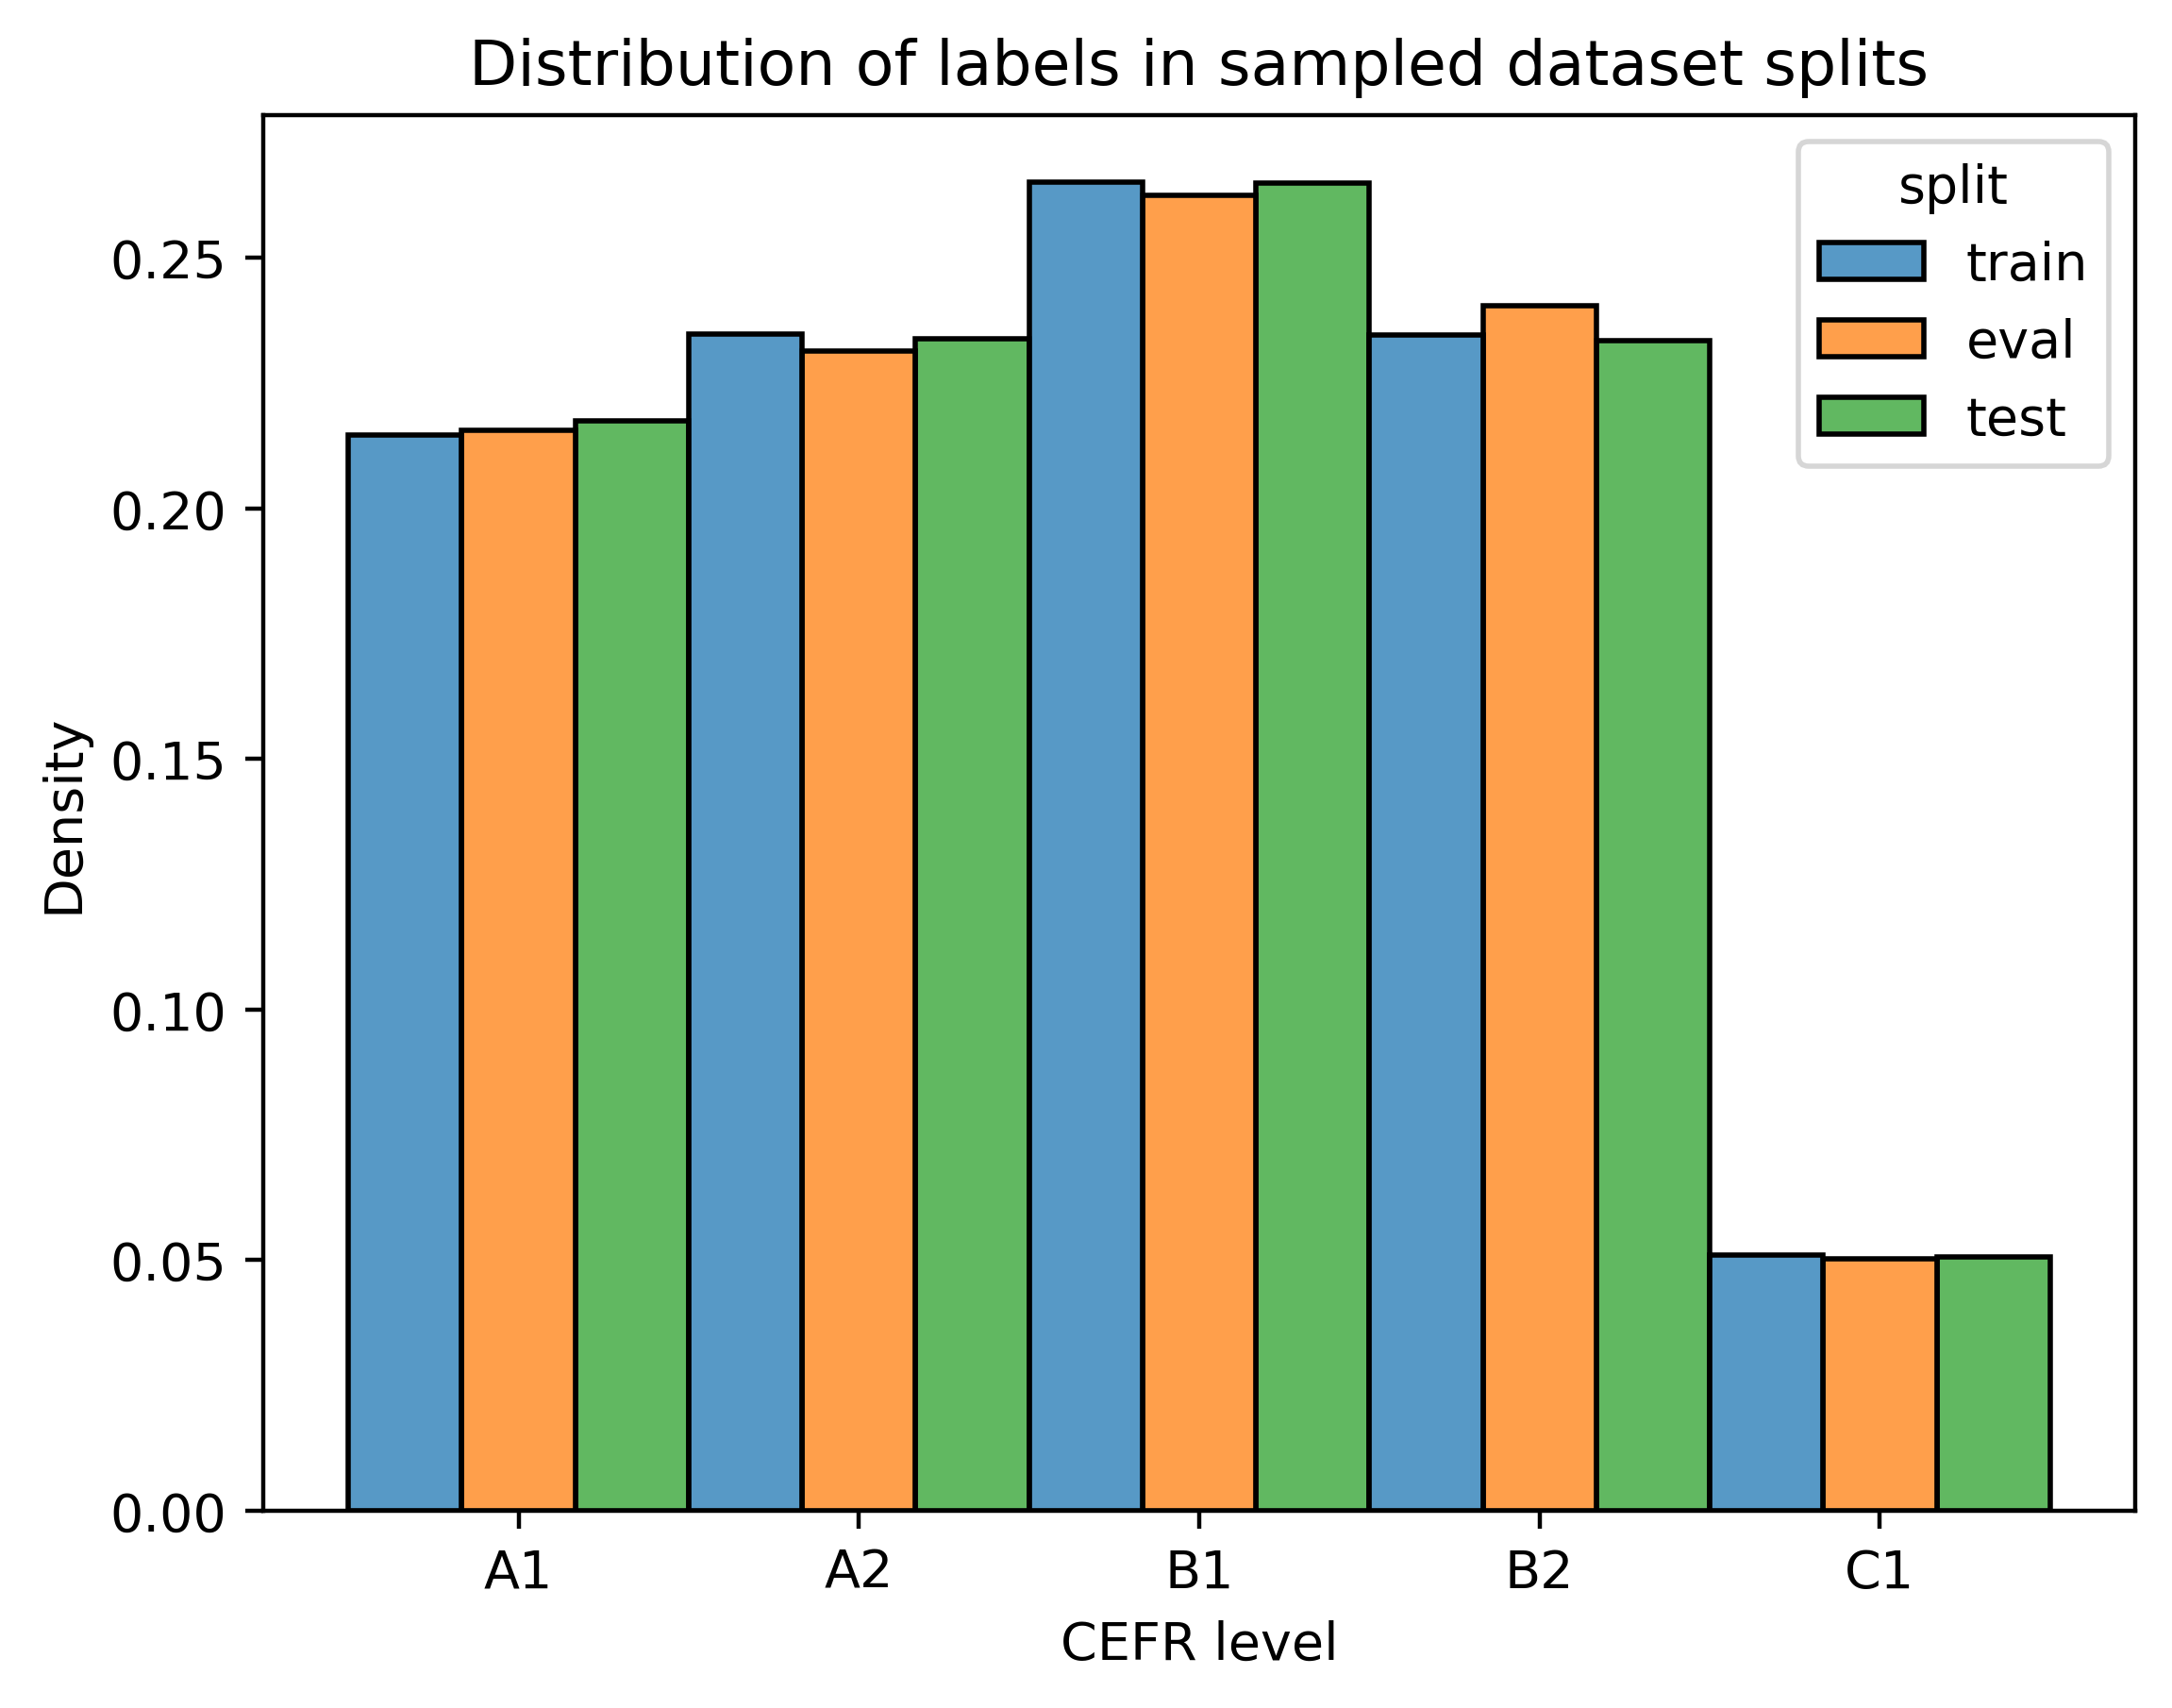
\includegraphics[width=0.8\textwidth]{figures/split-distributions-thinned.png}
  \caption{CEFR label distribution in the sampled dataset}
  \label{fig:cefr-distribution-sampled}
\end{figure}

\subsection{Using windowing technique in model predictions}

For model prediction, apart from just predicting on the whole text, I also
experimented with implementing the windowing technique. Rather than predicting
on the whole text, I would use the sliding window in the same way as described
earlier on the prediction text. Then I would have the model predict a label for
each window of the text and then aggregate together the labels into a single label
for the whole text. I experimented with multiple ways of aggregating together the
labels into a single one. The most straight-forward way would be to give the
text the label of the most frequently occurring label from the classifications
of the windows. However, the labels are the 1-16 Englishtown levels, which can
be considered a continuous scale. Due to this I also tried using the mean and
the median of the windows' classified labels to get a single label for the
whole text.

\section{Analysis/Results}



\section{Conclusion}

\printbibliography

\appendix

\section{More examples of texts from EFCAMDAT}

\begin{longtable}{l|p{0.85\textwidth}}
  \toprule
  Level & Text\\
  \midrule
  1 & Hi, everyone. This is the menu: Starter: Vegetables and cheese. Main
  course: Chicken and rice. Dessert: Ice cream. See you soon.\\
  \midrule
  2 & Tom and Cinthia, Welcome to Sao Paulo City. We are happy to have you
  here. There are many things you can do in the city. Take the buses 805, 807
  and 964 to go to the mall and the museum. In front of the mall you can see
  the tube station, take it and go to the beach, clear water's waiting for
  you.\%\% Beside home, in the evening, you can ask for pizza at number
  \#\#\#\#-\#\#\#\# and on the corner you can buy bread and milk at the bakery store. They sell
  book and newspaper there. On saturday morning you can go to the fair to eat
  some sneaks and have some fresh juice, a tipical Brazil juice. You and
  Cinthia will enjoy it. Kisses and have fun. \\
  \midrule
  4 & I was born in 1982. I got my first job when I was 20 years old. After I
  graduated from high school, I moved out of my parents' house. After I got an
  apartment, I got a good job. I met a girl at work and we fell in love. After
  I found a new job, we got married in 2008. Now we have a baby.\\
  \midrule
  6 & Dear Aunt Jane, An E-ticket is the ticket that shows your flight
  information. You can print it from your computer after you book your ticket.
  When you go to the airport, you can give the E-ticket and your passport to
  the attendant, then the attendant will help you to check in for the flight.
  Maybe you can ask for the aisle or window seat when you check in.\\
  \midrule
  8 & Hi Mr. Smith, I'd like to inform you that I have recently had a meeting
  with our business partner, Sally Cassidy. She was very friendly and
  optimistic. We discussed our cooperative project for the next year. It seems
  like a very lucrative and meaningful one. It's imperative to wrap up our
  current manufacturing process, so that we will be able to start the new one.
  Sally Cassidy invited me to visit their office and speak about the schedule
  tomorrow morning. However, I will keep you informed. Best regards, Tatiana\\
  \midrule
  10 & I had a meeting last week, actually was an interview for a new job. I
  was attend to be a trader in a big company here in my city. After
  introductions, (there was me, the export manager and one sales analyst), the
  manager asked me to talk a little bit about my experiences on my last
  position, I started with my graduation and how I migrated from tech to
  commercial department, then I described my experience with business in other
  countries. Here, they did some questions about how was my behavior in some
  situations, we started to talk about some cultures and behavior in different
  countries and then the manager explained what they expected from a new
  employee. He asked me if I was comfortable with this position and I said yes,
  then we talked about salary and he asked me on week to analyse and return to
  me.\\
  \midrule
  12 & I consider table manners important and I'm trying to teach them to my
  sons. Everyday, while we are eating at home, I ensure that they do not leave
  the table without permission, mine or my husband's, or, they do not ask for
  water without saying 'please' and 'thank you'. In particular, I want them to
  eat with their mouths closed, use the fork instead of taking the food with
  their hands and I don't want them to shout while we are at the table. When we
  are invited at somebody else's house for dinner, they behave really well.
  They want to carry and give the present we normally take to the hostess
  themselves, ask for permission to enter the house and never touch things
  around without seeking permission. What I want my sons to understand is that
  following some simple rules make them get more appreciated by the people
  surrounding them. They gain respect, too. My elder son has already understood
  that through politeness you can also respect the others' personal spaces and
  sensibilities. In Italy, many parents consider the education of children as a
  DIY activity. Not theirs, but their children's.\\
  \midrule
  13 & Unfortunately, green business is not so popular in my city. Citizens do
  not understand how important it is to use biodegradable and organic
  materials. I know only a few entrepreneurs who truly try to run a business to
  manufacture green products. My friend has an on-line shop of string bags for
  various categories of people such as housewife, business men, teenagers and
  etc. The bags may be cleaned and we have an opportunity not to use disposable
  plastic bags. Several companies made their offices with two sources of
  electricity there are an usual generator and solar panels. Their bills have
  become quite less. The second distinctive feature of these companies is
  digital devices instead of regular paper. Of course, in this case costs have
  become more. However, the local radio station interviews employees from these
  companies once a week in the evening program and the local newspaper
  publishes articles with surveys about their work conditions. So, by that
  companies got free advertisements. It is a balancing act to decide whether
  sustainability is essential or not for your business. But we are not only
  consumer of the planet's resources, we are part of it too.\\
  \midrule
  15 & Last year I was on a vacation in California. It was wonderful but one
  thing stays in my mind. People in America tend to communicate more indirectly
  compared with people in Germany, where I'm living. If you talk with someone
  you don't know you don't know if he says the truth or just wants to be nice
  to you. Sometimes this is really strange. But this is a foreign country with
  a different culture than what we have in Germany. Nevertheless I prefer
  direct communication although it's vulnerable. The kind of body language is
  similar to the one in Germany. There are no big differences.\\
  \bottomrule
  \caption{Example texts from EFCAMDAT at many Englishtown levels}
\end{longtable}

\section{More examples of texts from validation corpus}

\begin{longtable}{l|p{0.85\textwidth}}
  \toprule
  CEFR & Text\\
  \midrule
  A1 & My name's Annie Twigg and I'm a scientist. The chimpanzees in the photo are
  from Africa. They're a family. They're brothers and sisters. Their names
  are Tom, Brad, Keira and Angelina. They're happy. Their mother is in the
  photo too. Her name’s Meryl.\\
  \midrule
  A2 & My name's Cathy, and I'm an Aboriginal Australian. In the photo, I'm
  with my sister Emily. I'm the girl with the fringe. I'm 18 years old and I
  finished high school last year. My parents have a business and I work there.
  They make didgeridoos. The didgeridoo is a traditional instrument. Tourists
  buy them because they're great souvenirs. People are very surprised when they
  play a didgeridoo for the first time. They blow into it and it sounds really
  weird! I create beautiful designs on the didgeridoos. I love my job and I'm
  really happy when people like my designs.\\
  \midrule
  A2 & From: Julie\newline
  To: Alice\newline
  Hi,\newline
  Chloe arrived yesterday. She has long red hair, blue eyes and freckles. She's
  very nice, that's why she has lots of friends. She's chatty too, but
  sometimes she doesn't stop talking! I'm sure you will like her.\newline
  See you on Saturday!\newline
  Julie\newline
  xxx\\
  \midrule
  B1 & My name is Richard. All my life, I lived in New York City, but when I
  retired five years ago, I moved to Florida. I love it here! It’s sunny and
  beautiful every day of the year—and that means I can play golf every day.
  Golf is my favorite thing in life. I'm not far from the ocean, and I can go
  to the beach any time I want. It’s too bad that my children are all so far
  away, but they can visit me any time they want to. This is the perfect life
  for me!\\
  \midrule
  B2 & The world becomes better connected every day. It’s now easier than ever
  to keep in touch with friends and family around the world. Online banking
  allows people to access their accounts from anywhere that has an internet
  connection. People don’t even have to leave the house to go shopping!
  However, with greater connectivity comes greater risk. Every year, hundreds
  of thousands of people become victims of online crime. We asked our readers
  to share some of their terrible tech tales while we examine where the crimes
  originate.\\
  \midrule
  B2 & It is now over 50 years since the first publication of E.P. Torrance’s Tests of Creative Thinking, and they continue to be used worldwide as standard assessments of creativity.
  The tests typically consist of ‘divergent thinking’ tasks – the ability to
  generate a wide variety of solutions that are then scored on fluency,
  flexibility, originality and how fully explained they are. For example:\newline
  - Ways to improve: What could you do to make a toy truck more fun to play
  with?\newline
  - Imagine consequences: How would the world be different if everyone had an eye
  in the back of their head?\newline
  - Alternative uses: How many unusual uses for a brick can you think of?
  - Make drawings from a shape: Turn the Xs into pictures people might be
  surprised by. The X can be in any part of the picture. Add details to tell
  complete stories and give each picture a title.\newline
  Some question if the tests fully assess creativity because they say creativity is about originality and usefulness. Creativity not only requires divergent thinking but also ‘convergent thinking’ where you find one single solution that you feel is the best for the problem you are trying to solve.
  (...)\\
% Torrance followed the lives of children who first took his tests to see if they predicted creative achievements as adults. Analyses of these studies suggest they do. In fact, his tests are better at judging future creative success than intelligence tests. This is why they are frequently used to identify top managers in business and children for special educational programmes. It is also why there was concern in the USA when the magazine Newsweek reported that children’s scores on the tests were falling.
% Some have argued that this drop is because of children’s lifestyles: too many video games, too much TV and too little freedom to make choices. Others have suggested that education in the USA has become too focused on exam results, so teachers use fewer creative activities and favour more traditional learning by heart. This is in contrast to countries with a history of more traditional activities like memorization and practice drills such as China, which are doing the opposite and encouraging creativity through techniques such as problem-based learning.
% Problem-based learning involves setting a genuine problem such as reducing
% noise in a school library or deciding on a week’s menu of meals for an athlete.
% In reaching a conclusion, students have to do research across several subjects
% and be creative in the fullest sense. No doubt Torrance would have approved if
% he was still alive.\\
  \midrule
  C1 & An African in Greenland \newline
  One morning, when my brothers had left early for the coconut plantation, and
  there was no-one left at home to take me for a walk along the seashore, I went
  out alone and visited the Evangelical Bookshop. Inside there were two shelves
  against the walls on either side of the counter. I went up to one of these,
  attracted by a book laid flat on a half-empty shelf, with a cover showing a
  picture of a hunter dressed in clothes made of animal skins and leaning on a
  spear*. I was struck at once 15 by the title: The Eskimos* from Greenland to
  Alaska by Dr Robert Gessain. The book was illustrated with photographs and
  engravings*: I liked the look of it, bought it, then went on my way to the
  beach. By noon, I had finished my new book, the first I had read about the life
  of the little men of the north. Was it the author's praise of their hospitality
  that triggered my longing for adventure, or was it fear of returning to the
  sacred forest? I hardly remember. But when I had finished reading, one word
  began to resonate as inside me until it filled my whole being. That sound, that
  word was Greenland. In that land of ice, at least, there would be no snakes!\\
  \midrule
  C2 & Peer pressure exists across society, affecting people beneficially and adversely.
  In the case of the latter, certain risk factors have been identified that can make
  young people prone to undue, and often unwelcome, influence. When this occurs,
  there are strategies that can be used to handle the problem.
  Peers play an important role in a teenager's life as adolescence is the time
  when the desire to fit in and find acceptance and approval from the group is
  strongest. The need for approval is not bad in itself. It is part of what
  motivates adolescents to take extra care with their appearance, for instance.
  At times however, the desire to either impress or gain acceptance by the group
  becomes excessive, and can result in people choosing to take risks, with
  potentially serious consequences. Similarly, they might engage in behaviour
  that is extremely hurtful, like ridiculing someone with a physical or mental
  disability\\
  \bottomrule
\end{longtable}

\end{document}
